
%(BEGIN_QUESTION)
% Copyright 2011, Tony R. Kuphaldt, released under the Creative Commons Attribution License (v 1.0)
% This means you may do almost anything with this work of mine, so long as you give me proper credit

A pneumatic DP transmitter measures the flow of gasoline through a an orifice plate, using a separate square root extractor relay to characterize the signal so that it may be displayed linearly on the receiver gauge (FI-20):

$$\includegraphics[width=15.5cm]{i03440x01.eps}$$

Based on other flow-measuring devices in this process, operations personnel have determined the actual flow rate through this pipe is 158 gallons per minute.  FI-20, however, registers a flow of 142 gallons per minute.  Based on the data you see in this illustration, determine the location of the calibration error.

\underbar{file i03440}
%(END_QUESTION)





%(BEGIN_ANSWER)

The error lies either with the DP transmitter (FT-20), unequal fluid inside the impulse tubes, or with the orifice plate itself (FE-20).  One quick check would be to drain the impulse tubes (allowing fresh process gasoline to fill the tubes) and seeing whether that fixes the problem.  It's a quick procedure and it would eliminate that problem from the realm of possibility.

Another way to diagnose the problem is to remove FT-20 from service and test its calibration with applied pressures to its ``H'' side port.  If FT-20 checks out okay, the problem must be with the impulse tubes or the orifice plate.  

%(END_ANSWER)





%(BEGIN_NOTES)


%INDEX% Calibration errors, identifying
%INDEX% Measurement, flow: square root characterized pressure transmitter

%(END_NOTES)

